\listfiles
\documentclass{article}

\usepackage[pdftex]{graphicx}
\usepackage{amsmath}
\usepackage{amssymb}

\usepackage[a4paper,margin=1in]{geometry}

\newcommand{\half}{\frac{1}{2}}

\title{Heat capacity for moist porous solid}
\date{}

\begin{document}
\maketitle

\section{Pore contents}

\subsection{Mass of vapour}

According to the ideal gas law, the number of moles of vapour $n$ is

\begin{align*}
n = \frac{p_0 V}{RT_0}
\end{align*}

And since the molar mass $M$ is the mass per mole,

\begin{align*}
m_{s_0} &= Mn \\
&= \frac{MVp_0}{RT_0}
\end{align*}

\subsection{Mass of vapour and liquid water}

The mass of vapour is

\begin{align*}
m_s(T) &= Mn \\
&= \frac{MVp}{RT} \\
&= \frac{MV}{RT}p_0 e^{\frac{ML}{R}\left(\frac{1}{T_0} - \frac{1}{T}\right)}
\end{align*}

By conservation of mass,

\begin{align*}
m_s(T) + m_w(T) &= m_{s_0} + m_{w_0} \\
m_w(T) &= m_{s_0} + m_{w_0} - m_s(T) \\
&= \frac{MVp_0}{RT_0} + m_{w_0} - \frac{MV}{RT}p_0 e^{\frac{ML}{R}\left(\frac{1}{T_0} - \frac{1}{T}\right)}
\end{align*}

\subsection{Vapour mass change}

\begin{align*}
m_s(T) &= \frac{MV}{RT}p_0 e^{\frac{ML}{R}\left(\frac{1}{T_0} - \frac{1}{T}\right)} \\
\frac{d m_s(T)}{dT} &= \frac{d}{dT} \left(\frac{MV}{RT}p_0 e^{\frac{ML}{R}\left(\frac{1}{T_0} - \frac{1}{T}\right)}\right) \\
&= -\frac{MV}{RT^2}p_0 e^{\frac{ML}{R}\left(\frac{1}{T_0} - \frac{1}{T}\right)} + \frac{MV}{RT}p_0 e^{\frac{ML}{R}\left(\frac{1}{T_0} - \frac{1}{T}\right)}\frac{ML}{RT^2} \\
&= \frac{MV}{RT^2}p_0 e^{\frac{ML}{R}\left(\frac{1}{T_0} - \frac{1}{T}\right)} \left(\frac{ML}{RT} - 1\right)
\end{align*}

Hence

\begin{align*}
\Delta m_s(T) = \frac{MV}{RT^2}p_0 e^{\frac{ML}{R}\left(\frac{1}{T_0} - \frac{1}{T}\right)} \left(\frac{ML}{RT} - 1\right) \Delta T
\end{align*}

\subsection{Heat capacity of pore}

The number of moles of vapour is

\begin{align*}
n_s(T) &= \frac{m_s(T)}{M} \\
&= \frac{V}{RT}p_0 e^{\frac{ML}{R}\left(\frac{1}{T_0} - \frac{1}{T}\right)}
\end{align*}

The number of moles of liquid water is

\begin{align*}
n_w(T) &= \frac{m_w(T)}{M} \\
&= \frac{Vp_0}{RT_0} + \frac{m_{w_0}}{M} - \frac{V}{RT}p_0 e^{\frac{ML}{R}\left(\frac{1}{T_0} - \frac{1}{T}\right)}
\end{align*}

And the heat capacity is the sum of the heat capacity of the liquid and the heat capacity of the vapour

\begin{align*}
C_p(T) &= c_w n_w(T) + 3R n_s(T) \\
&= \frac{c_wVp_0}{RT_0} + \frac{c_w m_{w_0}}{M} - \frac{c_w V}{RT}p_0 e^{\frac{ML}{R}\left(\frac{1}{T_0} - \frac{1}{T}\right)} + \frac{3V}{T}p_0 e^{\frac{ML}{R}\left(\frac{1}{T_0} - \frac{1}{T}\right)}
\end{align*}

\subsection{Complete evarpouration}

The volume of the liquid water is $V_w = \delta V$, hence the mass is $m_{w_0} = \rho_w V_w = \rho_w \delta V$. Then the condition for complete evapouration is that $m_w = 0$ or

\begin{align*}
m_w(T) &= \frac{MVp_0}{RT_0} + m_{w_0} - \frac{MV}{RT}p_0 e^{\frac{ML}{R}\left(\frac{1}{T_0} - \frac{1}{T}\right)} \\
0 &= \frac{MVp_0}{RT_0} + \rho_w \delta V - \frac{MV}{RT}p_0 e^{\frac{ML}{R}\left(\frac{1}{T_0} - \frac{1}{T}\right)} \\
&= \frac{Mp_0}{RT_0} + \rho_w \delta - \frac{M}{RT}p_0 e^{\frac{ML}{R}\left(\frac{1}{T_0} - \frac{1}{T}\right)}
\end{align*}

Hence, letting $T = T_1$,

\begin{align*}
\frac{Mp_0}{RT_0} + \rho_w \delta &= \frac{M}{RT_1}p_0 e^{\frac{ML}{R}\left(\frac{1}{T_0} - \frac{1}{T_1}\right)} \\
e^{-\frac{ML}{RT_0}} \left( \frac{ML}{RT_0} + \frac{L \rho_w \delta}{p_0}\right) &= \frac{ML}{RT_1} e^{-\frac{ML}{RT_1}} \\
&= 1.305 \times 10^{-4}
\end{align*}

solving numerically,

\begin{align*}
\frac{ML}{RT_1} &= 11.38 \\
T_1 &= 438\mathrm{\ K}
\end{align*}

\subsection{Significant terms}

We consider the case where $T = T_0$, and $V = 0.1 \mathrm{\ cm^3}$ then

\begin{align*}
C_p(T) &= \frac{c_wVp_0}{RT_0} + \frac{c_w m_{w_0}}{M} - \frac{c_w V}{RT}p_0 + \frac{3V}{T}p_0 \\
\frac{c_wVp_0}{RT_0} &= 5.9 \times 10^{-4} \mathrm{\ J/K} \\
\frac{c_w m_{w_0}}{M} &= 6.6 \times 10^{-2} \mathrm{\ J/K} \\
\frac{c_w V}{RT}p_0 &= 5.9 \times 10^{-4} \mathrm{\ J/K} \\
\frac{3V}{T}p_0 &= 3.5 \times 10^{-6} \mathrm{\ J/K}
\end{align*}

As $T$ increase, however, the exponential term grows larger; hence we can keep the two largest terms and get

\begin{align*}
C_p(T) &= \frac{c_w m_{w_0}}{M} - \frac{c_w V}{RT}p_0 e^{\frac{ML}{R}\left(\frac{1}{T_0} - \frac{1}{T}\right)}
\end{align*}

The first term is the initial heat capacity of water and the second term is the capacity `lost' due to evapouration. It seems that the vapour does not contribute to the heat capacity and does not contain a lot of water.

\subsection{Specific heat capacity}

Since the total mass of pore content is always the same (water does not enter/exit the pore), the mass of pore content is

\begin{align*}
m_{s_0} + m_{w_0} &= \frac{MVp_0}{RT_0} + \delta \rho_w V
\end{align*}

and the specific heat capacity is

\begin{align*}
c_p(T) &= \frac{C_p(T)}{m_s + m_w} \\
&= \frac
{\frac{c_wVp_0}{RT_0} + \frac{c_w \delta \rho_w V}{M} - \frac{c_w V}{RT}p_0 e^{\frac{ML}{R}\left(\frac{1}{T_0} - \frac{1}{T}\right)} + \frac{3V}{T}p_0 e^{\frac{ML}{R}\left(\frac{1}{T_0} - \frac{1}{T}\right)}}
{\frac{MVp_0}{RT_0} + \delta \rho_w V} \\
&= \frac
{\frac{c_wp_0}{RT_0} + \frac{c_w \delta \rho_w}{M} - \frac{c_w}{RT}p_0 e^{\frac{ML}{R}\left(\frac{1}{T_0} - \frac{1}{T}\right)} + \frac{3}{T}p_0 e^{\frac{ML}{R}\left(\frac{1}{T_0} - \frac{1}{T}\right)}}
{\frac{Mp_0}{RT_0} + \delta \rho_w} \\
\end{align*}

for $T = T_0$,

\begin{align*}
c_p(T_0) &= \frac
{\frac{c_w \delta \rho_w}{M} + \frac{3}{T_0}p_0}
{\frac{Mp_0}{RT_0} + \delta \rho_w} \\
&= 231.1 \mathrm{\ J/gK}
\end{align*}

When $T > T_1$, there is no more water left and the terms that depend on $c_w$ sum to 0. Hence

\begin{align*}
c_p(T_1) &= \frac
{\frac{3}{T_1}p_0 e^{\frac{ML}{R}\left(\frac{1}{T_0} - \frac{1}{T_1}\right)}}
{\frac{Mp_0}{RT_0} + \delta \rho_w} \\
&= 3.10 \mathrm{\ J/gK}
\end{align*}

for $T > T_1$, since there is no further change to the composition of the pore (all of it is vapour), hence $c_p = 3.10 \mathrm{\ J/gK}$

\section{Porous solid}
\subsection{Specific heat capacity}
The mass of the solid body

\begin{align*}
m_S = (1 - \xi) \rho_S V_t
\end{align*}

where $V_t$ is the total body volume. Also,

\begin{align*}
V = \xi V_t
\end{align*}

Hence, if $H_S$ is the heat capacity of the body,

\begin{align*}
c(T) &= \frac{C_p(T) + H_S(T) }{m_s + m_w + m_S} \\
&= \frac
{\frac{c_w\xi V_tp_0}{RT_0} + \frac{c_w \delta \rho_w \xi V_t}{M} - \frac{c_w \xi V_t}{RT}p_0 e^{\frac{ML}{R}\left(\frac{1}{T_0} - \frac{1}{T}\right)} + \frac{3\xi V_t}{T}p_0 e^{\frac{ML}{R}\left(\frac{1}{T_0} - \frac{1}{T}\right)} + C_S (1 - \xi) \rho_S V_t}
{\frac{M\xi V_tp_0}{RT_0} + \delta \rho_w \xi V_t + (1 - \xi) \rho_S V_t} \\
&= \frac
{\frac{c_w\xi p_0}{RT_0} + \frac{c_w \delta \rho_w \xi }{M} - \frac{c_w \xi }{RT}p_0 e^{\frac{ML}{R}\left(\frac{1}{T_0} - \frac{1}{T}\right)} + \frac{3\xi }{T}p_0 e^{\frac{ML}{R}\left(\frac{1}{T_0} - \frac{1}{T}\right)} + C_S (1 - \xi) \rho_S }
{\frac{M\xi p_0}{RT_0} + \delta \rho_w \xi + (1 - \xi) \rho_S}
\end{align*}

\subsection{Numerical value}

\begin{align*}
c_p(T_0) &= 2591 \mathrm{\ J/kgK} \\
c_p(T_1) &= 111 \mathrm{\ J/kgK}
\end{align*}

For $T > T_1$, since the composition of the pore doesn't change, $c_p$ is still $111 \mathrm{\ J/kgK}$

\subsection{Graph}

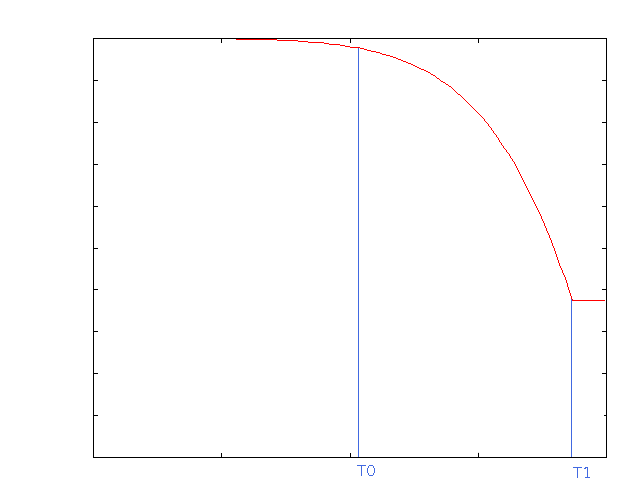
\includegraphics[width=\textwidth]{graphplot.png}

\end{document}
